\pagebreak

\section{Amplitude Shift Keying}
\label{sec:ask}

\subsection{Objective}
\label{sub:ask:Objective}
To understand the working of Amplitude Shift Keying (ASK) modulation and demodulation.

\subsection{Theory}
\label{sec:ask:theory}

Amplitude-shift keying is a form of amplitude modulation that represents digital data as variations in the amplitude of a carrier wave.

Any modulated signal has a high frequency carrier. The binary signal when ASK modulated, gives a zero value for Low input while it gives the carrier output for High input.


\subsection{MATLAB Code}
\label{sec:ask:matlab}

\inputminted[fontsize=\footnotesize,autogobble]{matlab}{code/ask.m}

\pagebreak
\subsection{Output}

\begin{figure}[ht]
	\centering
	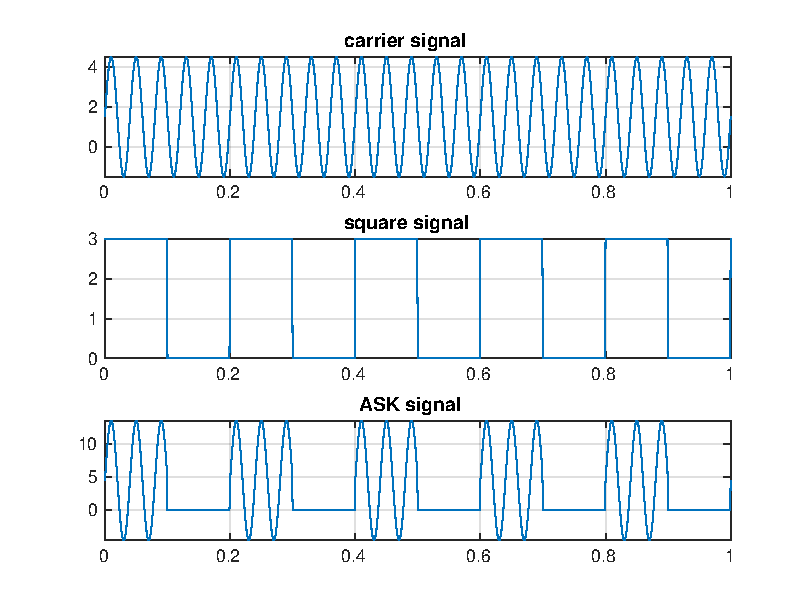
\includegraphics[width=0.6\textwidth]{res/figures/ASK.pdf}
	\caption{ASK Modulation}
	\label{fig:ask}
\end{figure}

